\section{Opgave 2 - Binary to 7-segment Hexadecimal - with case statement}
\begin{enumerate}
	\item[1)] Vi skriver koden med øvelse 4 i mente og udvider til hexadecimaler. Ud fra arket i øvelse 4 finder vi layout for 7-segment displayet og kreerer vores bogstaver:
\begin{lstlisting}[caption={Behavioral style binær til 7-segment hexadecimal},label={lst:binto7seghexa}]
library ieee;
use ieee.std_logic_1164.all;
use ieee.numeric_std.all;

entity binaryTo7SegHex is
port(A : in std_logic_vector(3 downto 0);
	segA : out std_logic_vector(6 downto 0));
end binaryTo7SegHex;

architecture selection of binaryTo7SegHex is
	begin
		process (A)
			begin
			case A is
				when "0000" => segA <= "0000001"; -- 0
				when "0001" => segA <= "1001111"; -- 1
				when "0010" => segA <= "0010010"; -- 2
				when "0011" => segA <= "0000110"; -- 3
				when "0100" => segA <= "1001100"; -- 4
				when "0101" => segA <= "0100100"; -- 5
				when "0110" => segA <= "0100000"; -- 6
				when "0111" => segA <= "0001111"; -- 7
				when "1000" => segA <= "0000000"; -- 8
				when "1001" => segA <= "0001100"; -- 9
				when "1010" => segA <= "0001000"; -- A
				when "1011" => segA <= "1100000"; -- B
				when "1100" => segA <= "0110001"; -- C
				when "1101" => segA <= "1000010"; -- D
				when "1110" => segA <= "0110000"; -- E
				when "1111" => segA <= "0111000"; -- F
				when others => segA <= "1111111"; -- Slukket
		end case;
	end process;
end selection;
\end{lstlisting}

\item[2)]
Vi illustrerer på følgende tre billeder vores program overført på DE2-boardet:
	\begin{figure}[h]
		\centering
		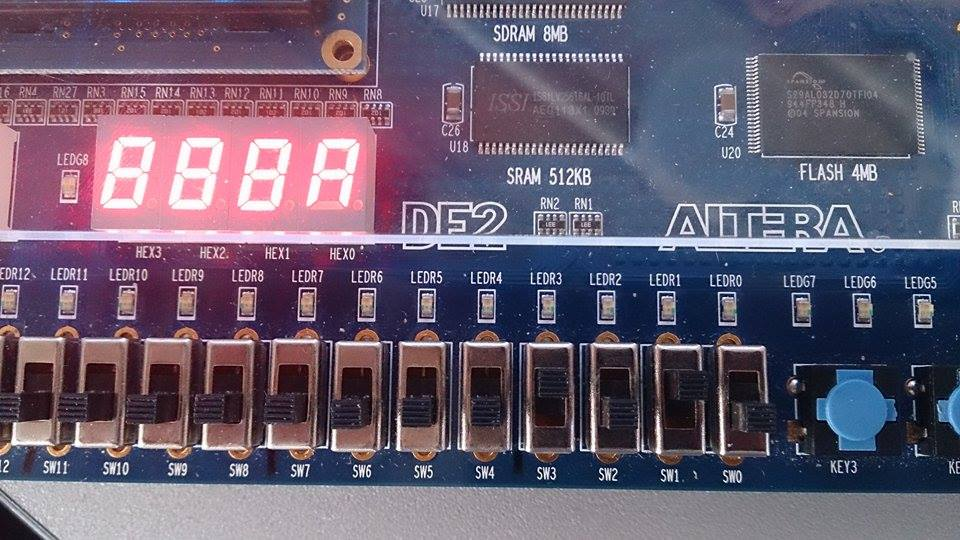
\includegraphics[scale=0.3]{pictures/Oevelse5/opg2/binTo7SegHexA.JPG}
		\caption{Tallet A}
		\label{fig:binTo7SegHexA}
	\end{figure}
	\begin{figure}[h]
		\centering
		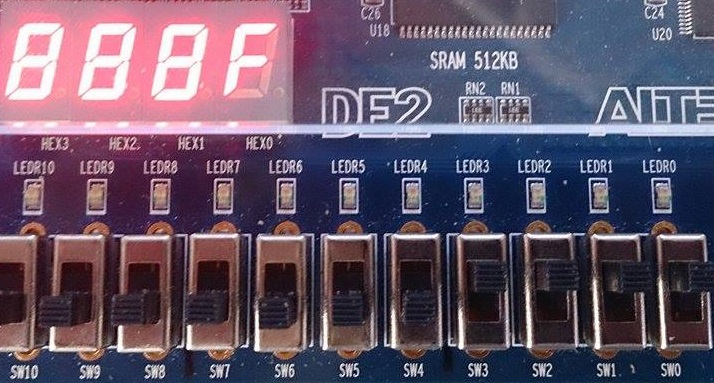
\includegraphics[scale=0.3]{pictures/Oevelse5/opg2/binTo7SegHexF.JPG}
		\caption{Tallet F}
		\label{fig:binTo7SegHexF}
	\end{figure}
	\begin{figure}[h]
		\centering
		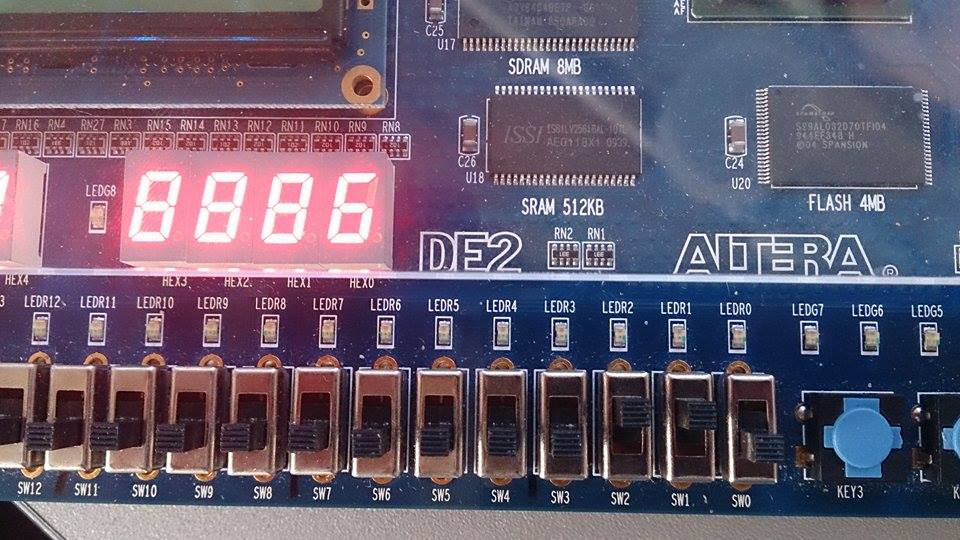
\includegraphics[scale=0.3]{pictures/Oevelse5/opg2/binTo7SegHex6.JPG}
		\caption{Tallet 6}
		\label{fig:binTo7SegHex6}
	\end{figure}
	